\documentclass{article}
\title{Whitepaper: Performance of Portable Faraday Cup Prototypes}
\author{Shaun Marshall, Blake Currier, Andrew Hodgdon}
\usepackage{amsmath}
\usepackage{amssymb}
\usepackage{nicefrac}
\usepackage{cancel}
\usepackage{anysize}
\usepackage{graphicx}
\usepackage{float}
\usepackage{subfigure}
\marginsize{1 in}{1 in}{1 in}{1 in}
\everymath{\displaystyle}
\begin{document}
\maketitle

\section{Introduction}
A model portable Faraday Cup (PFC) is being designed to calibrate proton accelerators, accurate to within 1\% error for therapy-range energies (70 to 250 MeV).  Preliminary investigations and implementations of the portable Faraday Cup were performed by Gottschalk et al (reference?).  The PFC will be a copper cylinder coated with a Kapton film to capture backscattered electrons.  The beam charge \emph{gain} (charge measured normalized to charge of beam) is acquired relative to a thin (12 micron) grounding layer of silver overlaying the Kapton film.  Charged particle transport within the Kapton layer contributes an effective image charge proportional to the depth into the PFC.  Dimensions of the copper cylinder and Kapton film thicknesses are optimized through evaluation of three models which emulate experimental trials.

\section{MCNP Optimization}
The height of the copper cylinder, whose central axis is in line with the source, must be sufficiently longer than the range of the protons at the upper limit of energies (6.3 cm @ 250 MeV); thus, 10 cm was used. \\

Fig.~\ref{fig:error_diameter} shows the variation of error (1-\emph{gain}) with copper diameter and method. Two methods are compared, SRIM (reference) and MCNP6. A conservative estimate of the error is found to drop below 1\% beyond a 6 cm diameter.  The same calculation was repeated with proton tallies alone, i.e., without any secondary electrons. This shows that if electrons had been completely ignored, the MCNP6 results would have been similar to the SRIM model and a diameter of 8 cm would have seemed reasonable.

\begin{figure}[H]
  \centering
  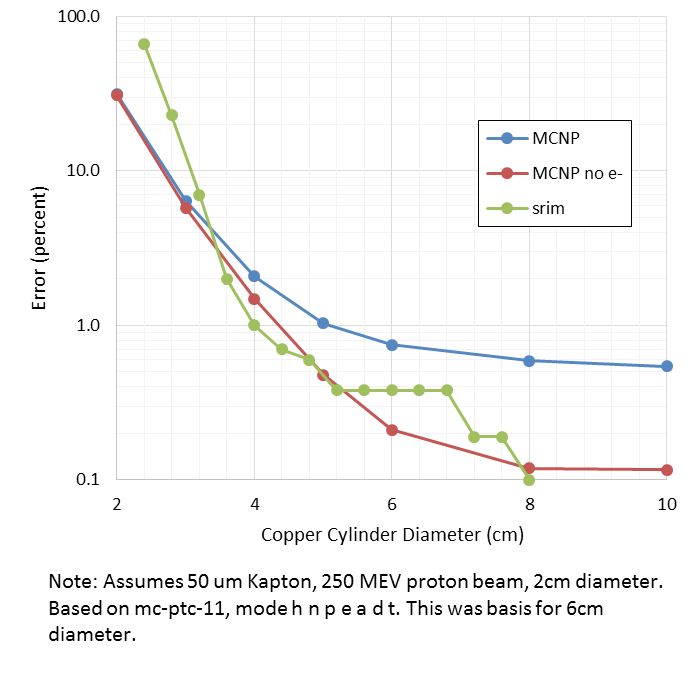
\includegraphics[width=6in]{figures/fig_error_diameter.png}
  \caption{Signal Error vs Diameter and Simulation Method} 
  \label{fig:error_diameter}
\end{figure}

\newpage
\section{Geant4 Optimization: In Vacuo}

To fully assess the behavior of backscattered electron capture in the Kapton film, three thicknesses were probed in accordance with experimental setups: 59, 100, and 200 microns.  Initially, an \emph{in vacuo} simulation of proton beam gain (w/ 1m events) is examined, with resulting gain measurements (fig.~\ref{fig:G4_results_vac}) for separate constructions with (+AgKA) and without (-AgKA) the outer grounding layer of Silver sheathed in additional Kapton.

\begin{figure}[H]
  \centering
  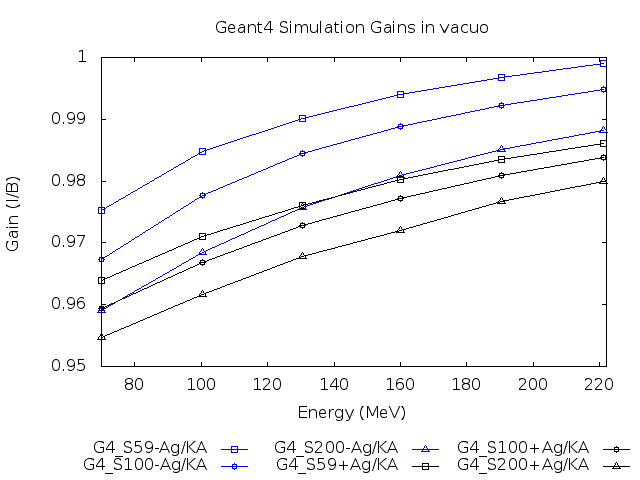
\includegraphics[width=5in]{figures/fig_G4_results_vac.png}
  \caption{\emph{In vacuo} comparison of PFC model gain via Geant4.  The blue lines (-AgKA) intersect with the black (+AgKA) at lower incident beam energies.} 
  \label{fig:G4_results_vac}
\end{figure}

Each increase in Kapton thickness lowers the overall gain measurement, indicative of captured backscattered electrons negatively contributing to the overall charge.  The grounding layer offsets this further, with the additional anomaly of converging gain measurements in the high energy limit across all three setups.  Indeed, charged partice transport histograms for these simulations (figs.~\ref{fig:G4_stats_vac_a}-~\ref{fig:G4_stats_AgKA_vac_c}) depict concentrations of depositions from the copper into the Kapton, but by a factor of 10 is outweighed by the contribution of charges (presumably electrons) \emph{entering} the copper.  Additionally, there is a buildup of charges in the shallow region of the Kapton, substantiating the flux of ions from the grounding layer and creating the gain anomaly.

\begin{figure}[H]
\centering
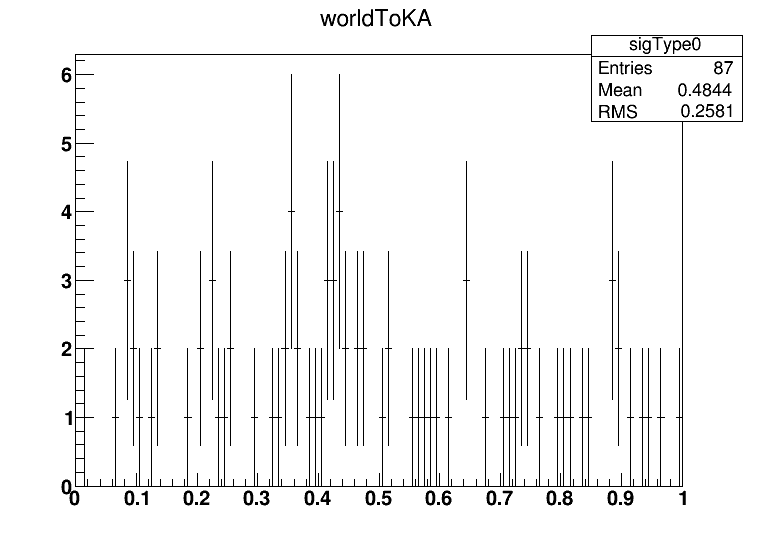
\includegraphics[width=6in]{figures/Cu_KA_vac/S59/WorldtoKA.png}
\caption{Terminus of charged particles at 250 MeV for 59 micron Kapton}
\label{fig:G4_stats_vac_a}
\end{figure}

\begin{figure}[H]
\centering
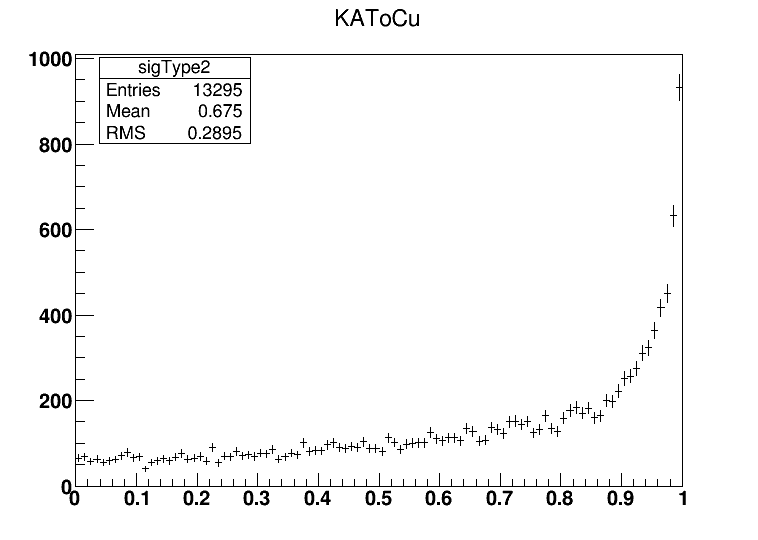
\includegraphics[width=6in]{figures/Cu_KA_vac/S59/KAtoCu.png}
\caption{Origin of charged particles at 250 MeV for 59 micron Kapton}
\label{fig:G4_stats_vac_b}
\end{figure}

\begin{figure}[H]
\centering
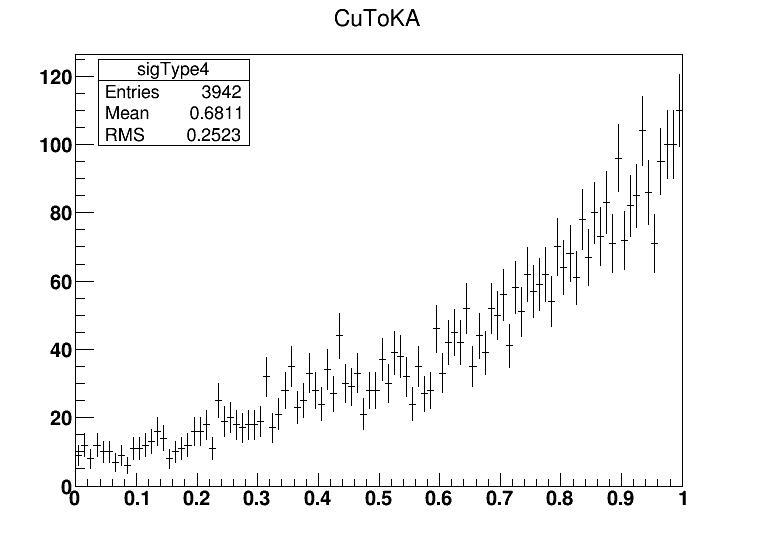
\includegraphics[width=6in]{figures/Cu_KA_vac/S59/CutoKA.png}
\caption{Terminus of charged particles at 250 MeV for 59 micron Kapton}
\label{fig:G4_stats_vac_c}
\end{figure}

\begin{figure}[H]
\centering
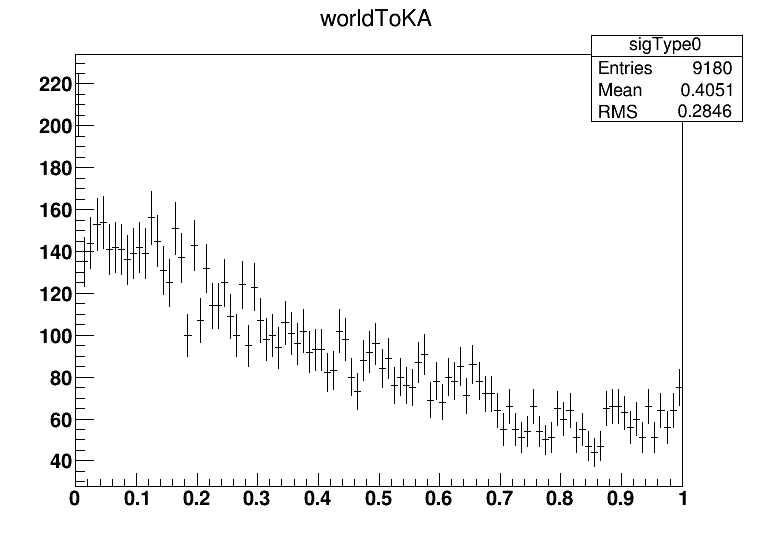
\includegraphics[width=6in]{figures/Cu_KA_AgKA_vac/S59/WorldtoKA.png}
\caption{Terminus of charged particles at 250 MeV for 59 micron Kapton with AgKA sheath}
\label{fig:G4_stats_AgKA_vac_a}
\end{figure}

\begin{figure}[H]
\centering
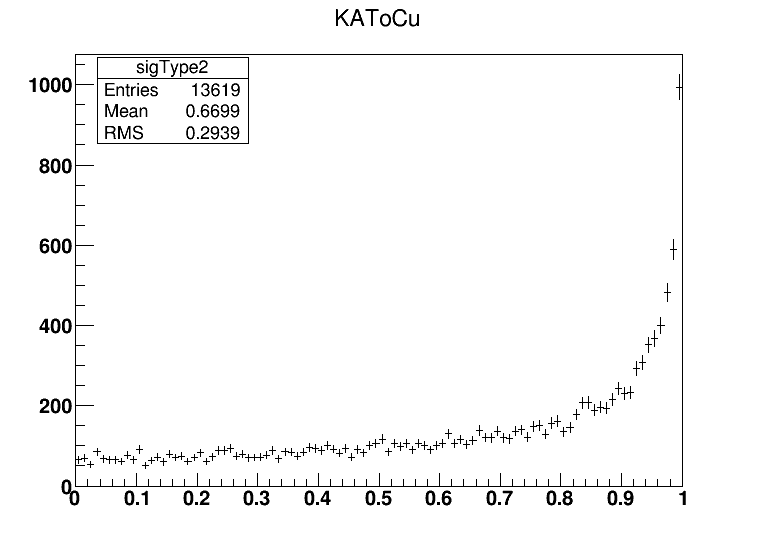
\includegraphics[width=6in]{figures/Cu_KA_AgKA_vac/S59/KAtoCu.png}
\caption{Origin of charged particles at 250 MeV for 59 micron Kapton with AgKA sheath}
\label{fig:G4_stats_AgKA_vac_b}
\end{figure}

\begin{figure}[H]
\centering
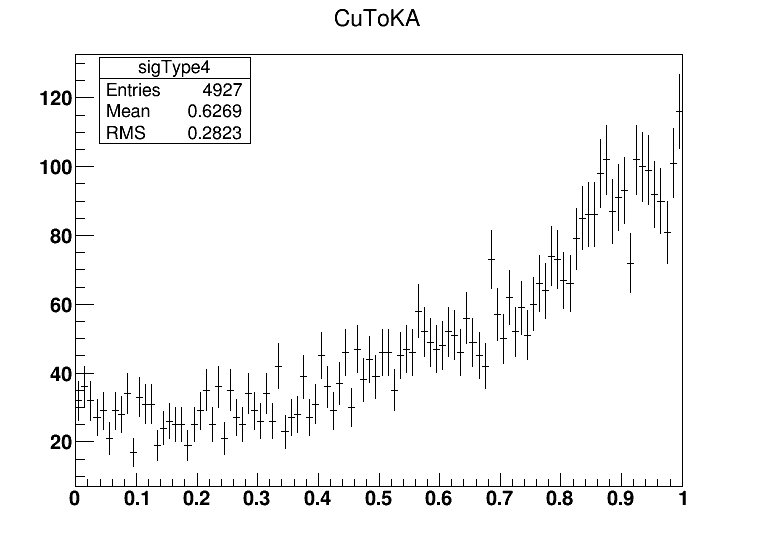
\includegraphics[width=6in]{figures/Cu_KA_AgKA_vac/S59/CutoKA.png}
\caption{Terminus of charged particles at 250 MeV for 59 micron Kapton with AgKA sheath}
\label{fig:G4_stats_AgKA_vac_c}
\end{figure}

\newpage
\section{Geant4 Optimization: In Air}

This processes is repeated for \emph{in air} measurements, with gain output in figure \ref{fig:G4_results_air}.  The same observations are made, though this time there is an exaggerated negativity at low energies without the grounding layer.

\begin{figure}[H]
  \centering
  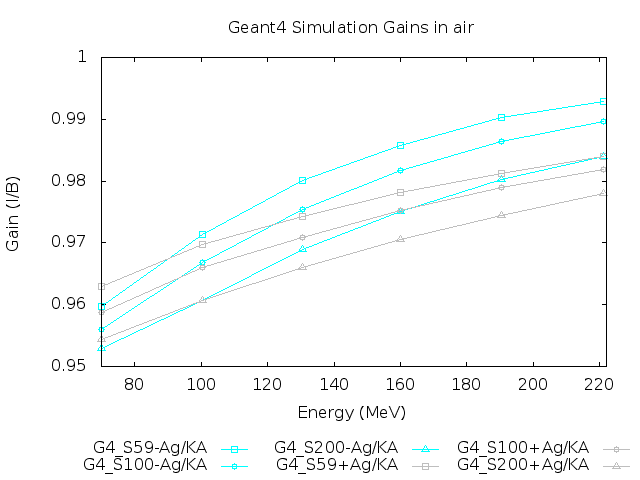
\includegraphics[width=5in]{figures/fig_G4_results_air.png}
  \caption{\emph{In air} comparison of PFC model gain via Geant4.  The blue lines (-AgKA) intersect with the black (+AgKA) at lower incident beam energies.} 
  \label{fig:G4_results_air}
\end{figure}

This is readily explained by figure \ref{fig:G4_stats_a}, where there is a buildup of charges from the air forced into the device by the primary particles.  This is \emph{not} seen in the subsequent setup with the Silver ground (fig.~\ref{fig:G4_stats_AgKA_a}), whose charged particle transport count is on the whole marginally greater than the \emph{in vacuo} equivalent.  This leads to the suspicion that the external Kapton sucessfully collected most of such stray charges from the air (histogram omitted). \\

The total overlaid plot is given in figure \ref{fig:G4_results}, including a pure copper control run.

\begin{figure}[H]
\centering
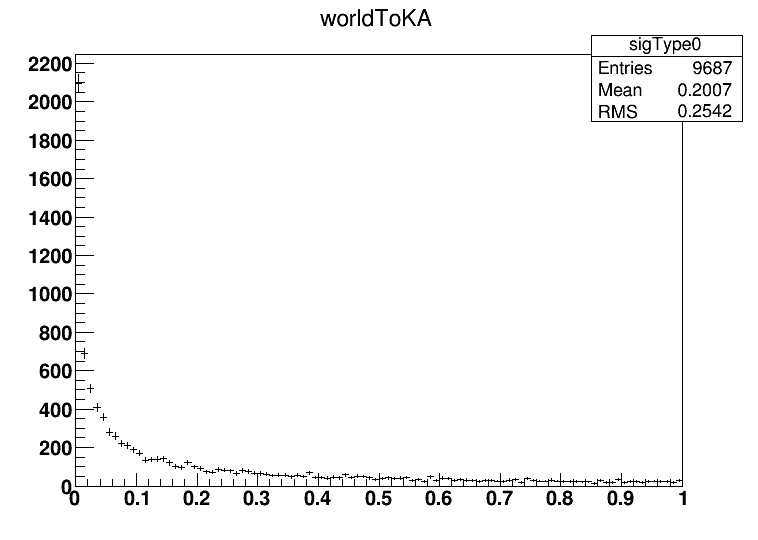
\includegraphics[width=6in]{figures/Cu_KA/S59/WorldtoKA.png}
\caption{Terminus of charged particles at 250 MeV for 59 micron Kapton}
\label{fig:G4_stats_a}
\end{figure}

\begin{figure}[H]
\centering
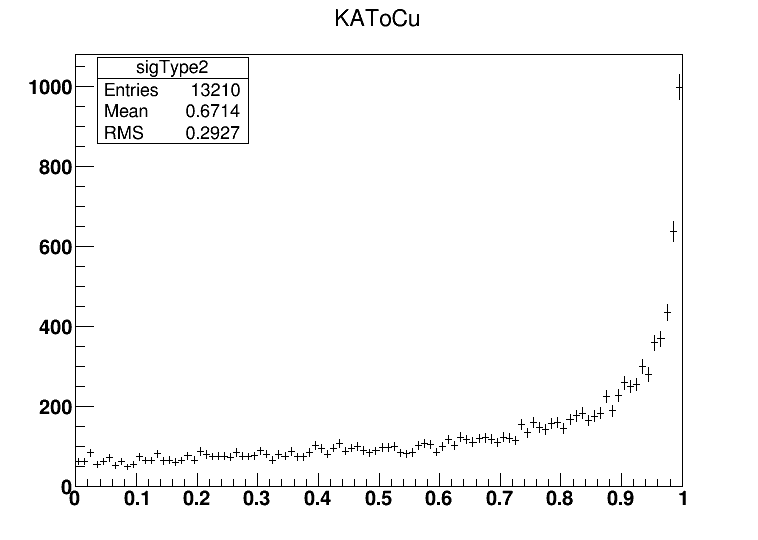
\includegraphics[width=6in]{figures/Cu_KA/S59/KAtoCu.png}
\caption{Origin of charged particles at 250 MeV for 59 micron Kapton}
\label{fig:G4_stats_b}
\end{figure}

\begin{figure}[H]
\centering
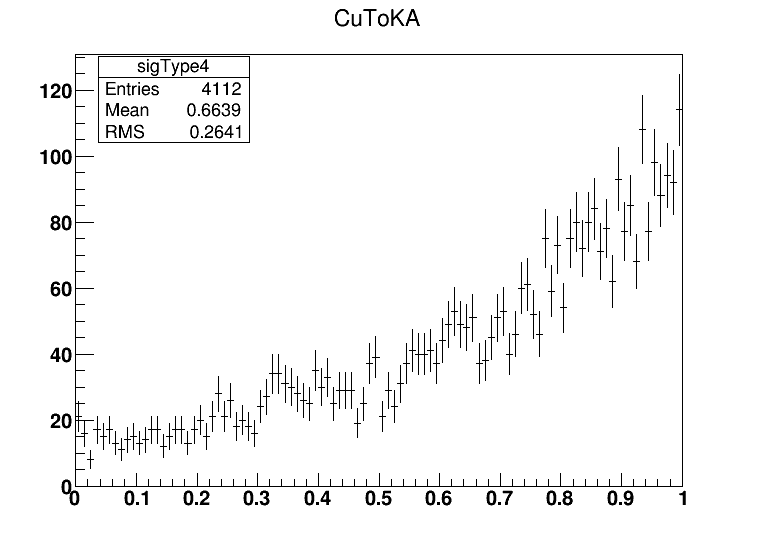
\includegraphics[width=6in]{figures/Cu_KA/S59/CutoKA.png}
\caption{Terminus of charged particles at 250 MeV for 59 micron Kapton}
\label{fig:G4_stats_c}
\end{figure}

\begin{figure}[H]
\centering
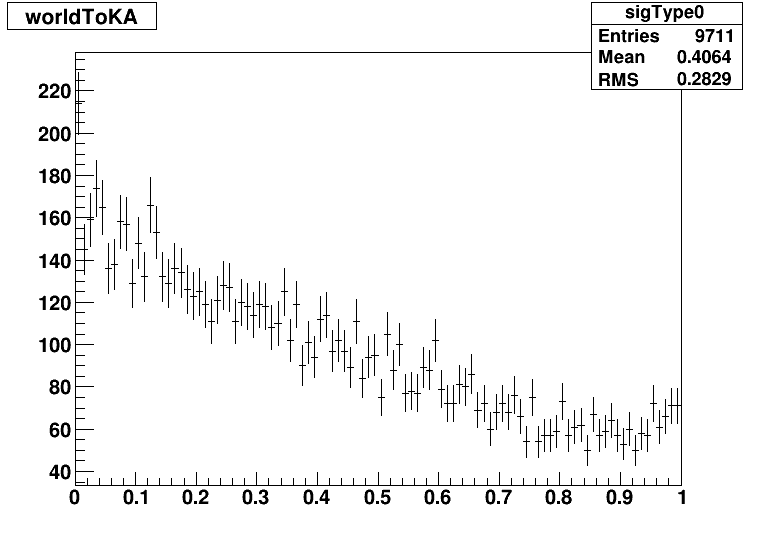
\includegraphics[width=6in]{figures/Cu_KA_AgKA/S59/WorldtoKA.png}
\caption{Terminus of charged particles at 250 MeV for 59 micron Kapton with AgKA sheath}
\label{fig:G4_stats_AgKA_a}
\end{figure}

\begin{figure}[H]
\centering
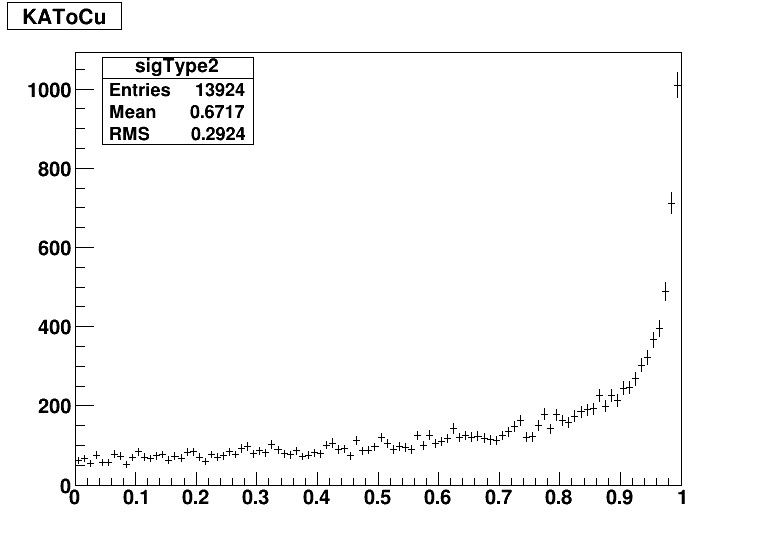
\includegraphics[width=6in]{figures/Cu_KA_AgKA/S59/KAtoCu.png}
\caption{Origin of charged particles at 250 MeV for 59 micron Kapton with AgKA sheath}
\label{fig:G4_stats_AgKA_b}
\end{figure}

\begin{figure}[H]
\centering
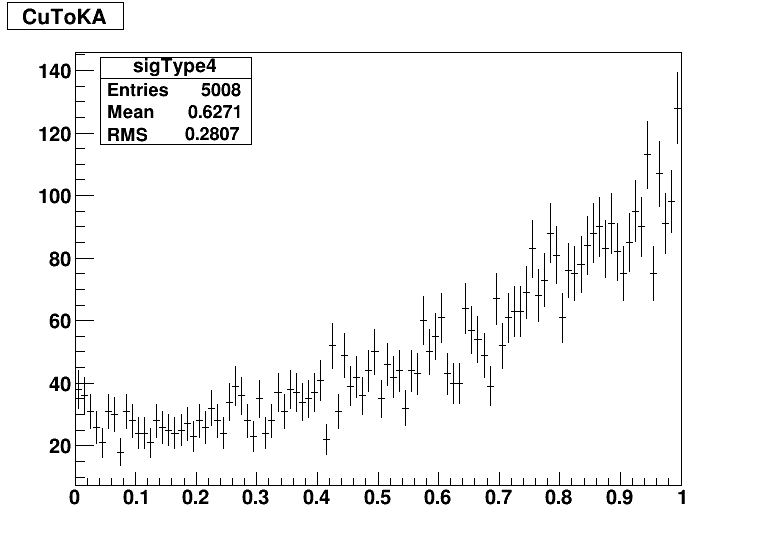
\includegraphics[width=6in]{figures/Cu_KA_AgKA/S59/CutoKA.png}
\caption{Terminus of charged particles at 250 MeV for 59 micron Kapton with AgKA sheath}
\label{fig:G4_stats_AgKA_c}
\end{figure}

\begin{figure}[H]
  \centering
  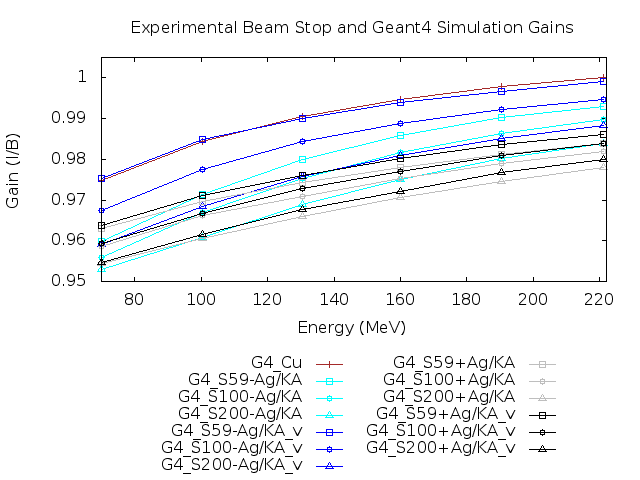
\includegraphics[width=5in]{figures/fig_G4_results.png}
  \caption{Comparison of PFC model gain via Geant4.} 
  \label{fig:G4_results}
\end{figure}

\begin{figure}[H]
  \centering
  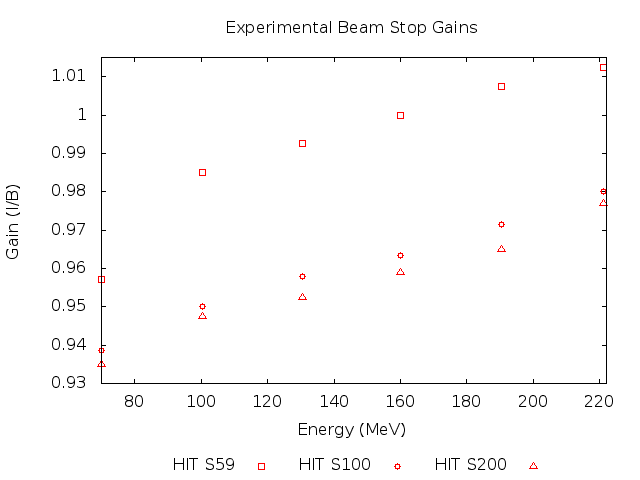
\includegraphics[width=6in]{figures/fig_HIT_results.png}
  \caption{Experimental data provided by the Heidelberg Institute of Technology for analogous prototypes} 
  \label{fig:HIT_data}
\end{figure}

\end{document}
